%%%%%%%%%%%%%%%%%%%%%%%%%%%%%%%%%%%%%%%%%%%%%%%%%%%%%%%%%%%%%%%%%%% 
%                                                                 %
%                            CHAPTER                              %
%                                                                 %
%%%%%%%%%%%%%%%%%%%%%%%%%%%%%%%%%%%%%%%%%%%%%%%%%%%%%%%%%%%%%%%%%%% 

\chapter{Software implementation with pure Smith-Waterman}

This capter will cover an approach to reference genome mapping using pure smith-waterman. This is a computationally very demanding task, but is more precise than heuristic methods such as FASTA, ...

\section{The concept}
For reference genome mapping a sequence of 75 to 300 bases in length should be mapped to the reference genome. The idea behind this mapping and the applications is thouroughly described in \ref{ch:algoverzicht}.

In this implementation, a mapping with "pure" Smith-Waterman was chosen. Commonly, an algorithm is used to select canditate locations where a small local smith-waterman is performed, or no smith waterman is performed at all. These methods are often less precise but computationally less demanding. Here, the alignment of the sequence is done with the full reference genome.

 //figuurtje


\section{General overview of the implementation}

\subsection{Parameters and Types}

\paragraph{Nucleotide base}
First of all, It seemed important to define the nucleotide bases. There are only 4 possible bases ($A$, $C$, $G$ and $T$), so 2 bits are enough. The following coding was chosen:

\begin{table}[H]
	\centering
	\begin{tabular}{|l|c|c|c|c|}
		\hline
		\textbf{Base} & A  & C  & G  & T  \\ \hline
		\textbf{Code} & 00 & 01 & 10 & 11 \\ \hline
	\end{tabular}
	\caption{\centering Encoding for the nucleotide bases}
\end{table}

To store these bases the uint8\_t type type from the stdint library was used. it is 1 byte in size which is the smallest available type in the C language. If more time would have been available, and an implementation with the full human genome would have been made, it might be a good idea to define a specific type consisting of only 2 bits, which would be a lot more memory efficient.

\paragraph{DNA sequence type} To easily keep track of a sequence in the program, a type was created which can hold a sequence of DNA. It consists of 2 parts: the length of the sequence and a pointer to the first base in memory. 
Since the genome can have a length of more than 3 billion bases, and the sequence is only a maximum of 300 bases in length, it made sense to use a separate type for the reference and for the sequence.\\

\begin{figure}[H]
	\centering
	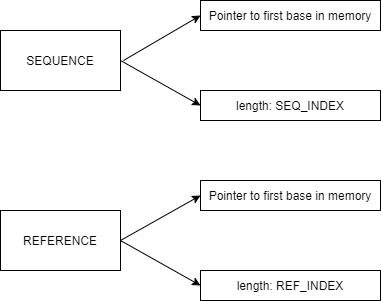
\includegraphics[width=0.35\textwidth]{systemImplementation/RefAndSeqTypes.png}
	\caption{The created types to store the sequence and the reference}
	\label{fig:RefAndSeqTypes}
\end{figure}

To index these "arrays" of bases, a new type was created for both the sequence indexing (\emph{SEQ\_INDEX}) and the reference indexing (\emph{REF\_INDEX}). Since an index to the sequence can be as high as the $length - 1$, it made sense to make the length attribute out of these newly created index types.

Since the //TODO echte types

\subsection{The code structure}

\begin{enumerate}
	\item Allocate some memory for the following data:
	\begin{enumerate}
		\item The reference genome, which can be quite large;
		\item current read;
		\item reverse complementary of current read;
		\item matrix for during the alignment. The amount of memory that should be allocated to this matrix is equal to the size of the sequence times the size of the reference.
	\end{enumerate}
	\item Initialize the first row and first column of the matrix on $0$, as it should be to perform the Smith-Waterman Algorithm;
	\item Load the reference genome from the fasta file;
	\item Open the FASTQ file for loading unmapped reads, and the SAM file to store the reads once they are mapped;
	\item For every read in the FASTQ file, we perform the following operations:
	\begin{enumerate}
		\item Load the next read from FASTQ file;
		\item Perform the alignment. (see \ref{expl:alignment});
		\item write the mapped read to the SAM file;
	\end{enumerate}
	\item Close the FASTQ and SAM files;
	\item free the reserved memory again
\end{enumerate}

\section{Details of the implementation}

As in most implementations in software, it was decided to split up the functionality of the program in multiple blocks. We have 3 big blocks:
\begin{enumerate}
	\item Interfacing with the memory: reserving memory for the used data, such as the reference, the sequence, and the alignment matrix.
	\item Interfacing with the files and the filesystem: Since the FASTA, FASTQ and SAM files are in a specific format, it made sense to build interpreters from and to these formats. 
	\item The alignment itself, which is the core of the program.
\end{enumerate}

\begin{figure}[H]
	\centering
	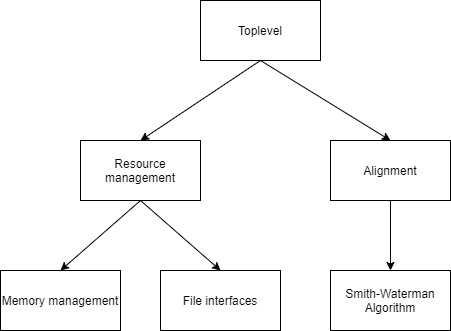
\includegraphics[width=0.5\textwidth]{systemImplementation/organigram.png}
	\caption{an organisation chart of the split up functionalities}
	\label{fig:organigram}
\end{figure}

\subsection{File interfaces}

\subsubsection{Parameters and types}

Since we need to interface FASTA, FASTQ and SAM files, it seemed appropriate to create 3 custom types. For the FASTA file, which stores the genome, the type \emph{GENOME} was created. In case of the FASTQ file and the SAM file, the respective types \emph{READ} and \emph{MAPPED\_READ} were created. Notice that the attributes of the types match the information to interface the files.

The information stored in the \emph{GENOME} type is the name of the genome (\emph{Rname}) and the reference.

\begin{figure}[H]
	\centering
	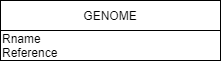
\includegraphics[width=0.35\textwidth]{systemImplementation/GenomeType.png}
	\caption{The type created to store the genome information.}
	\label{fig:GenomeType}
\end{figure}

In the \emph{READ} type, the current sequence is stored together with its quality string and its name.

\begin{figure}[H]
	\centering
	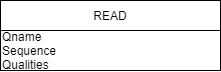
\includegraphics[width=0.35\textwidth]{systemImplementation/ReadType.png}
	\caption{The type created to store the read information}
	\label{fig:ReadType}
\end{figure}

The \emph{MAPPED\_READ} type contains all the information needed to write a full line in the SAM file, which is the output of the program.
Mark, the read itself is also stored in this type, since all the information in the read will also be written to the SAM file.

\begin{figure}[H]
	\centering
	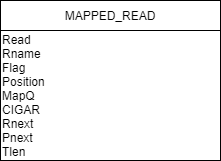
\includegraphics[width=0.35\textwidth]{systemImplementation/mappedReadType.png}
	\caption{The type created to store the mapping information, together with the read}
	\label{fig:mappedReadType}
\end{figure}

\subsubsection{Code structure}

First of all, the representation of the bases in the files (which is in the ASCII character format) should be transformable to the BASE type in the program. Because of this, conversion functions were created to change the character to base or vice versa.

\paragraph{FASTA interface} The function of this part is to load the genome from the FASTA file into the created \emph{GENOME} type. 
The FASTA file format is a simple text based way of storing a genome. On the first line is a '>' character followed by the name of the genome (\emph{Rname}). Starting from the second line to the end of the file the genome is stored. Often, this genome is split up using spaces or in multiple lines, so when coding the interpreter we need to make sure to skip these whitespace characters.

For better code readability, the genome loading is split into 2 functions that are be executed in order:
\begin{enumerate}
	\item loading the genome info
	\item loading the genome into the REFERENCE type. 
\end{enumerate}

\paragraph{FASTQ interface} this part of the program is responsible for loading the next read as a stream. The buildup of a FASTA file is thouroughly described in \ref{expl:FASTQ}.

In this case the code was also split up into functions for better readability:
\begin{enumerate}
	\item Loading the Qname, which is found on the first line for every read, behind a '@' character
	\item Loading the sequence, which is stored in a text based format in the FASTQ file, so it should be transformed to the SEQUENCE type. In a sequence it can happen that a base is suddenly marked with an 'N' character, which means after the primary processing the process was unable to identify the base. Because of the way the sequencing machines work, this only happens at the end of the sequence. So, it was decided to only cut the sequence short at the moment an 'N' character is registered.
	
	For example if the sequence were $ACGGCGCATTACNNAN$, the interface will only store $ACGGCGCATTAC$. This is justified by the fact that we are statistically certain that this sequence will be matched correctly from the moment the read is more than 15-20 bases long. The statistical proof itself will not be covered in this thesis.
	\item loading the qualities. Found on the fourth line for each read, the qualities for each base are stored. The information is stored in an array with the same length as the sequence.
	
\end{enumerate}


\paragraph{SAM interface} The SAM interface will write the current mapped read to a SAM file, one line for one read. The buildup of a SAM file is thouroughly described in \ref{expl:SAM}.

For this implementation, some values of the SAM format are not important and should be set to a default value. So it came naturally to create an "init" function, in which these default values are assigned. 
\begin{itemize}
	\item Rnext should be set to the '*' character;
	\item Pnext should be set to 0;
	\item Tlen should be set to 0;
\end{itemize}

Then, to write the line in the output SAM file, a function was created which accepts an attribute of the \emph{MAPPED\_READ} format and writes it as a line in the file.

\subsection{Memory management}

sdsalloc VS malloc
choosing sdsalloc so that hardware can also get it easily

\subsection{The alignment}
\label{expl:alignment}

\subsubsection{Parameters and types}

types!

\subsubsection{Code structure}

computational complexity: O(mn)

\section{Implementation results}

\subsection{Sample data}

PhiX 
galaxy
FASTQ: https://github.com/Illumina/Isaac3/tree/master/src/data/examples/PhiX/Fastq
coronavirus

//figuurtje IGV
uitleggen reading depth + sequence direction
desired result

\subsection{Results}

//figuurtje + bespreking
